\documentclass{article}

\usepackage[utf8]{inputenc}
\usepackage[spanish]{babel}

\usepackage{caratula}

\usepackage{graphicx}
\usepackage{subfig}
\usepackage{dirtytalk}
\usepackage{enumerate}

\usepackage{amssymb}
\usepackage{mathtools}
\usepackage{amsmath}
\usepackage{amsthm}

\usepackage{algorithm}
\usepackage{algpseudocode}
\usepackage{listingsutf8}

\usepackage{float}
\floatplacement{figure}{h!}

\usepackage{geometry}
\usepackage{fixltx2e}
\usepackage{wrapfig}
\usepackage{cite}
\usepackage{dsfont}

\usepackage[space]{grffile}

\geometry{
 a4paper,
 total={210mm,297mm},
 left=30mm,
 right=30mm,
 top=30mm,
 bottom=30mm,
 }
 
\newtheorem{theorem}{Teorema}[section]
\newtheorem{corollary}{Corolario}[theorem]
\newtheorem{lemma}{Lema}[theorem]
 
\theoremstyle{definition}
\newtheorem{definition}{Definición}[section]
 
\theoremstyle{remark}
\newtheorem*{remark}{Observación}
 
\begin{document}
% Estos comandos deben ir antes del \maketitle
\materia{Algoritmos y Estructuras de Datos III} % obligatorio

\titulo{Trabajo Práctico 3}
\subtitulo{}
\grupo{}

\integrante{Bayardo Julián}{850/13}{julian@bayardo.com.ar} % obligatorio
\integrante{Cuneo Christian}{755/13}{chriscuneo93@gmail.com} % obligatorio 
\integrante{Frassia Fernando}{340/13}{ferfrassia@gmail.com} % obligatorio 
\integrante{Gambaccini Ezequiel}{715/13}{ezequiel.gambaccini@gmail.com} % obligatorio 
 
\maketitle

\pagebreak

\tableofcontents

\pagebreak

\section{Problema 1}

El primer problema presenta un grafo a colorear en los que cada nodo tiene solo 1 o 2 colores posibles a elegir. A la hora de resolverlo pensamos reducir este problema a un problema ya resuelto. Para este caso especifico logramos ver que es posible transformar una instancia de este problema a una instancia de 2-Satisfiability.\par
Para conseguir esto necesitamos lograr convertir nuestra instancia en un conjunto de clausulas (que consisten de un OR entre varias variables o sus negaciones) tal que, si hay una asignación de estas variables que haga que todas las clausulas sean verdaderas, significa que nuestra instancia original tiene un coloreo valido. Y también necesitamos poder calcular este coloreo.\smallbreak
Entendiendo esto procedemos a buscar una forma correcta de crear una formula de lógica booleana a partir de una instancia del problema dado.\par
Cada nodo puede ser coloreado con uno o dos colores. 
En el caso que un nodo (llamémoslo A) tenga dos colores (digamos azul y rojo), tendremos las siguientes posibilidades:
\begin{enumerate}
\item A es rojo ($Ar$)
\item A no es rojo ($A\neg r$)
\item A es azul ($Aa$)
\item A no es azul ($A\neg a$)
\end{enumerate}
Naturalmente se deduce que $Ar \implies A\neg a$ y también $A\neg a \implies Ar$ ya que $A$ no puede estar coloreado con dos colores diferentes. Al mismo tiempo se tiene que $Aa \implies A\neg r$ y $A\neg r \implies Aa$ por lo mismo.

\begin{figure}
\centering
\begin{minipage}{0.45\textwidth}
\centering
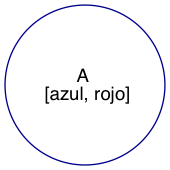
\includegraphics[width=3.5cm]{graphs/ej1/ej1_intro_2c.png}
\caption{first figure}
\end{minipage}\hfill
\begin{minipage}{0.45\textwidth}
\centering
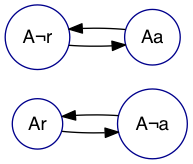
\includegraphics[width=3.5cm]{graphs/ej1/ej1_intro_2c_impl.png}
\caption{second figure}
\end{minipage}
\end{figure}


En el caso en que tenga solo un color (digamos azul) tenemos las siguientes posibilidades:
\begin{enumerate}
\item A es azul
\item A no es azul
\end{enumerate}
En este caso como es un único color necesitamos que este nodo este coloreado de este único color, por lo tanto la única implicación que siempre resulta en verdad es: $A\neg a \implies Aa$

\begin{figure}
\centering
\begin{minipage}{0.45\textwidth}
\centering
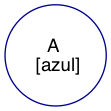
\includegraphics[width=2.5cm]{graphs/ej1/ej1_intro_1c.png}
\caption{first figure}
\end{minipage}\hfill
\begin{minipage}{0.45\textwidth}
\centering
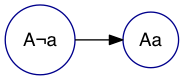
\includegraphics[width=3.5cm]{graphs/ej1/ej1_intro_1c_impl.png}
\caption{second figure}
\end{minipage}
\end{figure}

Luego, supongamos que hay dos nodos: $A$ que puede colorearse con azul y rojo, y $B$ que puede colorearse con azul. $A$ y $B$ son adyacentes.

Las implicaciones que vimos anteriormente siguen formando parte de la formula general, pero ahora los nodos son adyacentes y comparten un color en la lista de colores azul, por lo tanto tenemos que tener en cuenta que no pueden estar ambos nodos coloreados de este color al mismo tiempo. De esto ultimo generamos unas nuevas implicaciones: $Aa \implies B\neg a$ y $Ba \implies A\neg a$.

\begin{figure}
\centering
\begin{minipage}{0.45\textwidth}
\centering
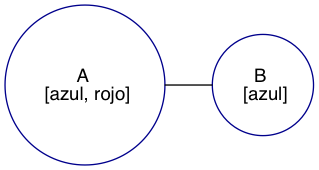
\includegraphics[width=5cm]{graphs/ej1/ej1_intro_2na.png}
\caption{first figure}
\end{minipage}\hfill
\begin{minipage}{0.45\textwidth}
\centering
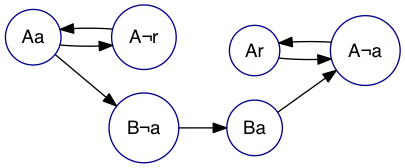
\includegraphics[width=6cm]{graphs/ej1/ej1_intro_2na_impl.png}
\caption{second figure}
\end{minipage}
\end{figure}

Si en cambio tenemos dos nodos: $A$ que puede colorearse con azul y verde, y $B$ que puede colorearse con rojo, y estos son adyacentes, no habría ninguna implicación mas que tener en cuenta

\begin{figure}
\centering
\begin{minipage}{0.45\textwidth}
\centering
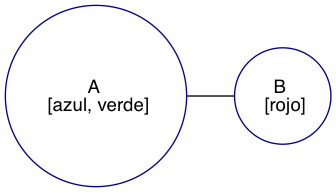
\includegraphics[width=5cm]{graphs/ej1/ej1_intro_2n.png}
\caption{first figure}
\end{minipage}\hfill
\begin{minipage}{0.45\textwidth}
\centering
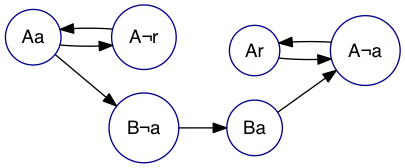
\includegraphics[width=6cm]{graphs/ej1/ej1_intro_2n_impl.png}
\caption{second figure}
\end{minipage}
\end{figure}


\section{Problema 2}

Para resolver de manera exacta el problema de List Coloring decidimos implementar un algoritmo de backtracking que recorra todas las soluciones parciales posibles, y deje sin explorar las soluciones parciales que no llevarán a una solución final válida. Esto es, coloreando cada nodo con cada color posible para él y explorando el espacio de soluciones que esto genera. 

Para asegurarnos que, a priori, todas las soluciones válidas están contempladas podemos ver que una solución válida requiere a cada nodo pintado de alguno de los colores que éste admita (\textit{propiedad 1}) y que además cada nodo no repita color con sus vecinos (\textit{propiedad 2}). Veamos luego que, dado un nodo, estamos coloreándolo con cada color que admite, y para cada color hacemos lo mismo con los nodos restantes; en otras palabras, al generar cada permutación de colores estamos cumpliendo la \textit{propiedad 1} -porque cada nodo está pintado con alguno de sus colores- y como son todas las posibles, si hay coloreo que cumpla la \textit{propiedad 2}, ciertamente está dentro de todas las permutaciones generadas. 

Para optimizar nuestro algoritmo y reducir el costo de explorar soluciones inválidas, decidimos chequear al momento de colorear un nodo($u$) si su color a evaluar($c$) está en conflicto con sus vecinos ya coloreados, dado que de ser así, ésta automáticamente deja de constituir parte de una solución válida; por lo que optamos por no pintar $u$ con $c$, y seguimos adelante en su lista de colores.  
Notemos que esto no elimina soluciones posibles, dado que por definición, un coloreo válido de los nodos de un grafo $G(V,E)$, es una asignación $f$: $V$ $\rightarrow$ $C$, tal que $f(u)$ $\neq$ $f(v)$ $\forall$ $(u,v)$ $\in$ $E$ y como vimos que $u$ pintado con $c$ ya no cumplen dicha propiedad, cualquier coloreo que lo contenga pintado de este color no será una solución válida. También notemos que como consecuencia de esta poda, de llegar a terminar de iterar por todos los nodos (habiéndole asignado un color a cada uno), tal coloreo constituye un coloreo válido. Esto se puede demostrar trivialmente, dado que de no ser un coloreo válido habríamos podado esta rama con anterioridad, con lo cual es absurdo haber coloreado todos los nodos si el coloreo resultante no fuese válido. 

Además, como parte de la consigna, en cada una de las soluciones parciales generadas, chequeamos si la instancia es reducible a un problema de 2-List Coloring, dado que de ser así, podemos utilizar el algoritmo propuesto en el \textbf{Problema 1} y obtener una solución a dicha instancia en tiempo polinomial. 

\begin{algorithm}
\caption{Algoritmo de backtracking}
\label{ex2:pseudo1}

\begin{algorithmic}
\Function{coloringExists}{graph, colors, current, node}
\If{current.complete()} \Comment $O(1)$
    \State \Return current; \Comment $O(1)$
\Else
    \If{is2ListColoring(graph, colors, current)} \Comment $O(n)$
        \State 2ListColoring(graph, transform(graph, colors, current)); \Comment $ O(n + List Coloring)$
    \EndIf
    \For{colour $\in$ colors.get(node)}
        \If{isAdmissible(graph, current, node, colour)} \Comment $O(n)$
            \State current.set(node, colour) \Comment $O(1)$
            \State \textbf{try} \Comment $O(1)$
            \State \indent \Return coloringExists(graph, colors, current, node+1)
            \State \textbf{catch(...)} \Comment $O(1)$
            \State \indent continue;
        \EndIf
    \EndFor
    \State \textbf{throw error} \Comment $O(1)$
\EndIf
\EndFunction
\end{algorithmic}
\end{algorithm}


Para el algoritmo de chequeo de instancia de 2-List Coloring, recorremos todos los nodos del grafo, y verificamos que cada uno cumpla estar coloreado o no estarlo pero además admitir un máximo de dos colores posibles. Es fácil ver cómo esta verificación cumple con una instancia de un problema de 2-List Coloring: 
\begin{enumerate}
\item Para los nodos ya coloreados, por la poda mencionada en el algoritmo \ref{ex2:pseudo1}, estos ya presentan un coloreo válido y el mismo continua siéndolo.
\item Para los nodos no coloreados, cumplen la precondición del problema de 2-List Coloring de que todos admitan un máximo de dos colores.
\end{enumerate}


\begin{algorithm}
\caption{Chequeo de instancia de 2ListColoring}
\label{ex2:pseudo2}

\begin{algorithmic}
\Function{is2ListColoring}{graph, colors, current}
\For{node $\in$ graph} \Comment $O(n)$
    \If{!current.isset(node) $\wedge$ colors.get(node).size() $>$ 2} \Comment $O(1)$
        \State \Return false; \Comment $O(1)$
    \EndIf
\EndFor
\State \Return true; \Comment $O(1)$
\EndFunction
\end{algorithmic}
\end{algorithm}


Finalmente, para la transformación de una instancia de problema de List Coloring a uno de 2-List Coloring, es necesario entender que se cumple la precondición de el algoritmo \ref{ex2:pseudo2}. Siendo así, sabemos que todos los nodos cumplen estar coloreados, o no estarlo pero tener como máximo dos colores en sus colores permitidos. Con lo cual, la transformación se reduce a, en caso que sea necesario, limitar los colores que cada nodo admite.
Dicho esto, la transformación es: para cada nodo, en caso de estar coloreado, reducir sus colores posibles al color con el que está pintado; y de lo contrario, admitir su lista de colores tal como está.
Esto cumple ser una instancia válida de 2-List Coloring, dado que cada nodo admite dos colores como máximo, y además preservamos la solución parcial otorgada por el algoritmo \ref{ex2:pseudo1}.


\begin{algorithm}
\caption{Transformación de instancia}
\label{ex2:pseudo3}

\begin{algorithmic}
\Function{transform}{graph, colors, current}
\State $var$ ColorStorage: $output$($graph$.size()) \Comment $O(n)$
\For{vertex $\in$ graph} \Comment $O(n)$
    \If{colors.get(vertex).size() $\leq$ 2} \Comment $O(1)$
        \State $output$.add(vertex, colors.get(vertex)) \Comment $O(1)$
    \Else
        \State $output$.add(node, current.get(vertex)) \Comment $O(1)$
    \EndIf
\EndFor
\State \Return $output$ \Comment $O(1)$
\EndFunction
\end{algorithmic}
\end{algorithm}

\subsection{Análisis de Complejidad}
Para analizar la complejidad del algoritmo, veamos que, a priori, generamos todas las permutaciones posibles de colores, con lo cual las complejidades en peor y mejor caso dependerán de cómo esté compuesto nuestro grafo y de cuántos colores admita cada nodo.

Notemos que en peor caso, nuestro grafo tiene $n$ nodos, es completo y cada nodo admite los $c$ colores posibles, además $c$ debe ser mayor que 2, dado que así la instancia no será reducible a una de 2-List Coloring. Con lo que, en nuestro árbol de \textit{backtracking}, abriremos $c$ ramas para cada nodo, lo que a priori hace a la complejidad O($c^{n}*f(n)$), siendo $f(n)$ el costo de todas las operaciones auxiliares. Dicho costo adicional es el generado por \textit{is2ListColoring} y \textit{isAdmissible}, el cual es $\theta$($n$) - dado que en \textit{is2ListColoring} iteramos sobre todos los nodos del grafo una vez y las operaciones auxiliares son constantes, y en \textit{isAdmissible} iteramos sobre todos los vecinos del nodo actual (los cuales en este caso son n-1 nodos) y las operaciones auxiliares también son constantes-, haciendo que la complejidad se torne O($n*c^{n}$).

En mejor caso, se considera un grafo sin aristas, dado se puede pintar trivialmente asignando cualquier color admisible a cada nodo. En este caso, el algoritmo \ref{ex2:pseudo1} recorrería cada nodo exactamente una vez y lo pintaría del primer color en su lista. Notemos que esto no generará conflicto con sus vecinos, dado que no los tiene, y además al terminar de recorrer el último nodo, se tiene un coloreo válido (porque todos están coloreados y no hay colisiones). Esto sugiere que la complejidad se torna O($n*f(n)$).
En cuanto a las funciones auxiliares, veamos que ahora \textit{isAdmissible} tiene complejidad constante, porque no hay vecinos por los cuales iterar y comparar. Sin embargo, \textit{is2ListColoring} mantiene su complejidad de peor caso, porque sin importar las aristas del grafo, el algoritmo \ref{ex2:pseudo2} siempre recorre todos los nodos, por lo que su complejidad sigue siendo $\theta$($n$). Habiendo dicho esto, podemos concluir que la complejidad de las funciones auxiliares es O($n$), determinando así la complejidad del mejor caso que es O($n^{2}$).

\section{Problema 3}

El problema 3 pedía que desarrollemos una heurística golosa para el problema
de list coloring. La heurística que decidimos aplicar es la de ordenar los nodos de manera descendente por grado, y a su vez, ordenar la lista de colores de cada nodo de manera descendente por frecuencia, para luego iterar desde el de mayor grado al de menor, eligiendo el color que menos conflictos generase. Si algún color al momento de ser elegido genera 0 conflictos, se elige ese color para ese vértice y se prosigue al siguiente vértice. 
La idea es que al setear los colores de los nodos de mayor grado con los colores más frecuentes se generasen menos conflictos a futuro y a su vez se minimice la cantidad de colores total a usar.

La complejidad de la heurística es $O(N^{2}C)$, ya que hay que recorrer $O(N)$ vértices, y por cada vértice, recorrer todos sus colores, ($O(C)$ en peor caso), y a su vez, para cada color, calcular la cantidad de conflictos del vértice con sus vecinos, que pueden ser a lo sumo $O(N)$.

El caso de un grafo completo es el peor posible, porque todos los nodos tienen que tener un color diferente, siendo la complejidad final $O(N^{2}C)$.
En cambio, en familias de grafos conocidas que tengan un número cromático $K$ constante, es posible que la heurística tenga una complejidad de $O(N^2 * K)$, que finalmente es $O(N^2)$ al ser $K$ constante.



\begin{algorithmic}
\Function{greedyOrder}{graph, colorStorage}
\State colors = colorStorage.sortByFrequency() \Comment $O(N*C)$
\State vertexOrder = graph.descendingByDegree() \Comment $O(N Log(N))$
\State coloring = ConflictColoring(graph)
\For{v $\in$ vertexOrder}  \Comment $O(N)$
    \State choice = 0
    \State conflicts = $\infty$
    \For{c $\in$ colors[v]}        \Comment $O(C)$
        \State coloring.setu(v, c) \Comment $O(N)$
        \State currentConflicts = coloring.conflicts(v) \Comment $O(1)$
        \If{currentConflicts $<$ conflicts}
            \State choice = c
            \State conflicts = currentConflicts
            \If{currentConflicts $==$ 0}
                \State break
            \EndIf
        \EndIf
    \EndFor
    \State coloring.setu(v, choice) \Comment $O(N)$
\EndFor
\State \Return coloring
\EndFunction
\end{algorithmic}










\section{Problema 4}

En términos del problema 4, a priori el algoritmo de búsqueda local es la misma metaheuristica que nos dieron en clase. Como solución inicial tomamos a la solución generada por la heurística del problema 3, y procedemos a realizar la búsqueda local de la forma indicada en clase, visible en el algoritmo \ref{ex4:pseudo1}.

\begin{algorithm}
\caption{Algorítmo de búsqueda local}
\label{ex4:pseudo1}

\begin{algorithmic}
\State current $\gets$ ejercicio3()
\While{1}
    \State next $\gets$ neighbour(current, graph, colors)
    
    \If{current $\leq$ next}
        \State return current
    \Else
        \State current $\gets$ next
    \EndIf
\EndWhile
\end{algorithmic}
\end{algorithm}

Donde la función neighbour nos dice el mejor de los vecinos de la instancia pasada por parámetro. A priori, es claro que este programa termina: dado que neighbour siempre debería devolver al menor de los vecinos, siempre estamos siguiendo una cadena de instancias decrecientes por el criterio de comparación; además, está implícito que todo el conjunto de posibles vecindades de una instancia tiene al menos un mínimo, por lo que eventualmente deberíamos converger hacia el mismo. En términos de las vecindades, optamos por elegir las siguientes heurísticas:

La primer vecindad, visible en el algoritmo \ref{ex4:pseudo2}, considerada consiste en tomar los $k$ vértices con mayor número de colisiones con sus vecinos, y para cada uno de ellos probar con absolutamente todos los colores que no sean el actualmente asignados, tomando como vecino final a aquel cuyo cambio de color genere el menor número de colisiones globales finales. En el caso en que ningún cambio mejore la cantidad de colisiones finales, simplemente nos quedamos con la instancia inicial.

\begin{algorithm}
\caption{Primer vecindad}
\label{ex4:pseudo2}

\begin{algorithmic}
\Function{neighbour}{original, graph, colors}
    \State size $\gets \min(|V(\text{graph})|, k)$ \Comment $O(1)$
    \State conflicts $\gets$ Conflictos por vértice de original \Comment $O(n + m)$
    \State queue $\gets$ min-queue() \Comment $O(1)$
    
    \For{$n \in \{0, .., \text{size}\}$} \Comment $O(k log(k))$
        \State queue.push($\langle$conflicts[$n$], $ n\rangle$) \Comment $O(log(k))$
    \EndFor
    
    \For{$n \in \{\text{size}, .., |V(\text{graph})|\}$} \Comment $O((n - k) log(k))$
        \State current $\gets$ queue.top() \Comment $O(1)$
        
        \If{$\pi_1$(current) $<$ conflicts[$n$]} \Comment $O(1)$
            \State queue.pop() \Comment $O(log(k))$
            \State queue.push($\langle$conflicts[$n$], $ n\rangle$) \Comment $O(log(k))$
        \EndIf
    \EndFor
    
    \State best $\gets$ original \Comment $O(n)$
    
    \For{$n \in \{0, .., \text{size}\}$} \Comment $O(cn + log(k))$
        \State vertex $\gets$ $\pi_2($queue.top()$)$ \Comment $O(1)$
        \State queue.pop() \Comment $O(log(k))$
        \State old $\gets$ color del vértice vertex en el coloreo original \Comment $O(1)$
        
        \For{color admisible para el vértice vertex} \Comment $O(cn)$
            \If{color $\neq$ old} \Comment $O(1)$
                \State next $\gets$ original \Comment $O(n)$
                \State next.set(vertex, color) \Comment $O(n)$
                \If{next.conflicts() $<$ best.conflicts()} \Comment $O(1)$
                    \State best $\gets$ next \Comment $O(n)$
                \EndIf
            \EndIf
        \EndFor
    \EndFor
    
    \Return best
\EndFunction
\end{algorithmic}
\end{algorithm}

La segunda vecindad, en algoritmo \ref{ex4:pseudo2}, consiste en tomar al nodo cuya relación entre cantidad de colisiones con sus vecinos y su grado sea la mayor en todo el grafo, y luego probar con todos los cambios de colores posibles para este nodo, tomando como instancia final aquella que minimice la cantidad de colisiones del nodo elegido con sus vecinos. Una vez más, en el caso en que ningún cambio mejore la cantidad de colisiones finales, simplemente nos quedamos con la instancia inicial.

\begin{algorithm}[h]
\caption{Segunda vecindad}
\label{ex4:pseudo2}

\begin{algorithmic}
\Function{neighbour}{current, graph, colors}
    \State best $\gets$ 0 \Comment $O(1)$
    \State ratio $\gets$ 0 \Comment $O(1)$
    
    \For{$i \in \{0, .., |V(graph)|\}$} \Comment $O(n + m)$
        \State current $\gets$ $\frac{\text{current.conflicts}(i)}{\text{graph.degree}(i)}$ \Comment $O(n + m)$ la primera vez, $O(1)$ luego
        
        \If{current $>$ ratio} \Comment $O(1)$
            \State ratio $\gets$ current \Comment $O(1)$
            \State best $\gets$ i \Comment $O(1)$
        \EndIf
    \EndFor
    
    \State initial $\gets$ current.color(best) \Comment $O(1)$
    \State conflicts $\gets$ current.conflicts(best) \Comment $O(1)$
    
    \For{color $\in$ colors.get(best)} \Comment $O(cn)$
        \If{color $\neq$ initial} \Comment $O(1)$
            \State previous $\gets$ current.color(best) \Comment $O(1)$
            \State current.set(best, color) \Comment $O(n)$
            
            \If{current.conflicts(best) $<$ conflicts} \Comment $O(1)$
                \State conflicts $\gets$ current.conflicts(best) \Comment $O(1)$
            \Else
                \State current.set(best, previous) \Comment $O(n)$
            \EndIf
        \EndIf
    \EndFor
    
    \Return current
\EndFunction
\end{algorithmic}
\end{algorithm}

Cabe destacar que en el caso de la primera heurística el criterio que determina la mejoría de una instancia con respecto a otra es la cantidad de colisiones a nivel global (a pesar de que el cambio sea a nivel local), mientras que en el caso de la segunda es la cantidad de colisiones del nodo contra sus vecinos, que es un criterio local. Como criterio de comparación entre instancias, decidimos tomar el indicador que nos resultó más natural para determinar qué tan buena es una instancia: la cantidad de colisiones a nivel global. Esto quiere decir que en cada paso, la búsqueda local sólo puede mejorar la solución en términos de cantidad de colisiones globales, garantizándonos de esta forma que al finalizar poseemos un mínimo local bajo este criterio.

En términos de la implementación, dado que en este caso necesitamos acceder muy frecuentemente a información sobre los conflictos a nivel global y entre vecinos, utilizamos una representación con información sobre la cantidad de conflictos de cada vértice con el coloreo actual, y cambiamos las operaciones para que cada actualización del coloreo mantenga actualizada esta información adicional de manera acorde.

\subsection{Análisis de Complejidad}

Es importante hablar primero sobre la implementación de un coloreo que realizamos: originalmente, la estructura de un coloreo consistía básicamente en un arreglo con una asociación de colores para cada nodo y un valor reservado particular que indicaba la falta de un color en los casos en que fuera necesario. Sin embargo, la gran cantidad de cálculos con respecto a la cantidad de conflictos que presentaban las heurísticas nos hicieron considerar una alternativa ligeramente más sofisticada: en la implementación actual, poseemos además un arreglo que indica la cantidad de colisiones de cada nodo con sus vecinos, así como una variable que cuenta la cantidad de colisiones a nivel global, y una variable adicional que indica si el arreglo está actualizado. Esta representación nos permite garantizar una complejidad temporal de $O(1)$ al obtener los conflictos cuando el arreglo está actualizado, y nos fuerza a realizar una actualización (que nos toma $O(n + m)$) en los casos en que no lo está. Además, agregamos una variante de la operación de coloreo que nos permite realizar la actualización al momento en que se realiza la operación, costando un total de $O(dg(v)) = O(n)$ en el peor caso.

En el caso de la primera vecindad, no es muy complicado el análisis de complejidad: los primeros dos ciclos acumulan un total de $O(n log(k))$ pasos en conjunto, y el último de los ciclos basta con ver el código para encontrase con que la complejidad es $O(cn + nlog(k))$, haciendo que en total tengamos $O(n(c + log(k)))$ tras considerar todas las operaciones. 

En el caso de la segunda vecindad, tomar el grado de un nodo es una operación $O(1)$ y todas las otras realizadas en el primer ciclo también lo son. Por lo que la complejidad temporal es $O((n + m) + (n - 1)) = O(n + m)$ para el primer ciclo, donde el primer término proviene de la primer iteración, y el segundo de todas las otras juntas. Luego, en términos del segundo ciclo, el mismo se realiza a lo sumo $c$ veces, y en el peor caso ningún cambio de color mejora la cantidad de conflictos, por lo que terminamos realizando $O(2n) = O(n)$ operaciones en cada iteración, por un total de $O(cn)$ en todo el ciclo. Finalmente, la complejidad del algoritmo para obtener el mejor vecino es $O(n + m + cn) = O(cn + m)$ (aunque cabe destacar que en realidad ese $O(cn)$ es una cota grosera para la complejidad real, que es $O(c * dg(best))$; pensamos que esta cota más ajustada podría servirnos cuando realicemos el análisis de mejor y peor caso con hipótesis adicionales sobre los grados de los nodos).

Pensemos, entonces, qué sucede con la búsqueda local. En el mejor caso, el resultado del ejercicio 3 es un mínimo local de antemano, en cuyo caso vamos a estar ejecutando una única vez la iteración de la búsqueda, encontrando que no hay mejoría y saliendo de esta forma. En el peor caso, el resultado del ejercicio 3 tiene exactamente $m$ conflictos (es el caso en el que todos los nodos tienen el mismo color), y asumiendo que bajamos de a exactamente un conflicto hasta llegar al óptimo de cero conflictos, tenemos exactamente $m$ iteraciones de la vecindad. Por lo tanto, en el peor caso tendríamos $O(mn(c + log(k)))$ para la búsqueda local con la primer vecindad, y $O(m(cn + m))$ para la segunda vecindad.

Sin embargo, según la experimentación que realizamos, la heurística del ejercicio 3 tiende a tener muy buenos resultados con las clases de grafos conocidas que utilizamos, por lo que no pudimos determinar claramente qué grafos nos resultarían en un peor caso del algoritmo (ya que a priori precisaríamos forzar a la heurística golosa a generar un resultado sumamente malo, para que las búsquedas locales se vean forzadas a correr múltiples veces). Por lo tanto, la forma de probar mejor y peor caso es básicamente comenzar la búsqueda local de mejor caso con un coloreo que sea un mínimo local y comenzar con un coloreo donde todos los nodos tengan el mismo color, respectivamente.

%% TODO: GRAFICOS PEOR Y MEJOR CASO'

\subsection{Análisis de efectividad}



\section{Código fuente}

\lstset{inputencoding=utf8/latin1}
\lstset{basicstyle=\footnotesize\ttfamily,breaklines=true}
\lstset{framextopmargin=50pt,frame=bottomline}

\subsection{Main}
%\lstinputlisting[language=C++]{../src/main.cpp}

\subsection{Ejercicio 1}
%\lstinputlisting[language=C++]{../src/Exercise1.h}
%\lstinputlisting[language=C++]{../src/Exercise1.cpp}

\subsection{Ejercicio 2}
%\lstinputlisting[language=C++]{../src/Exercise2.h}
%\lstinputlisting[language=C++]{../src/Exercise2.cpp}

\subsection{Ejercicio 3}
%\lstinputlisting[language=C++]{../src/Exercise3.h}
%\lstinputlisting[language=C++]{../src/Exercise3.cpp}

\subsection{Ejercicio 4}

\end{document}